\documentclass{standalone}
\usepackage{tikz}
\usetikzlibrary{patterns, positioning}
\usepackage[sfdefault]{ClearSans} %% option 'sfdefault' activates Clear Sans as the default text font
\usepackage[T1]{fontenc}

\begin{document}
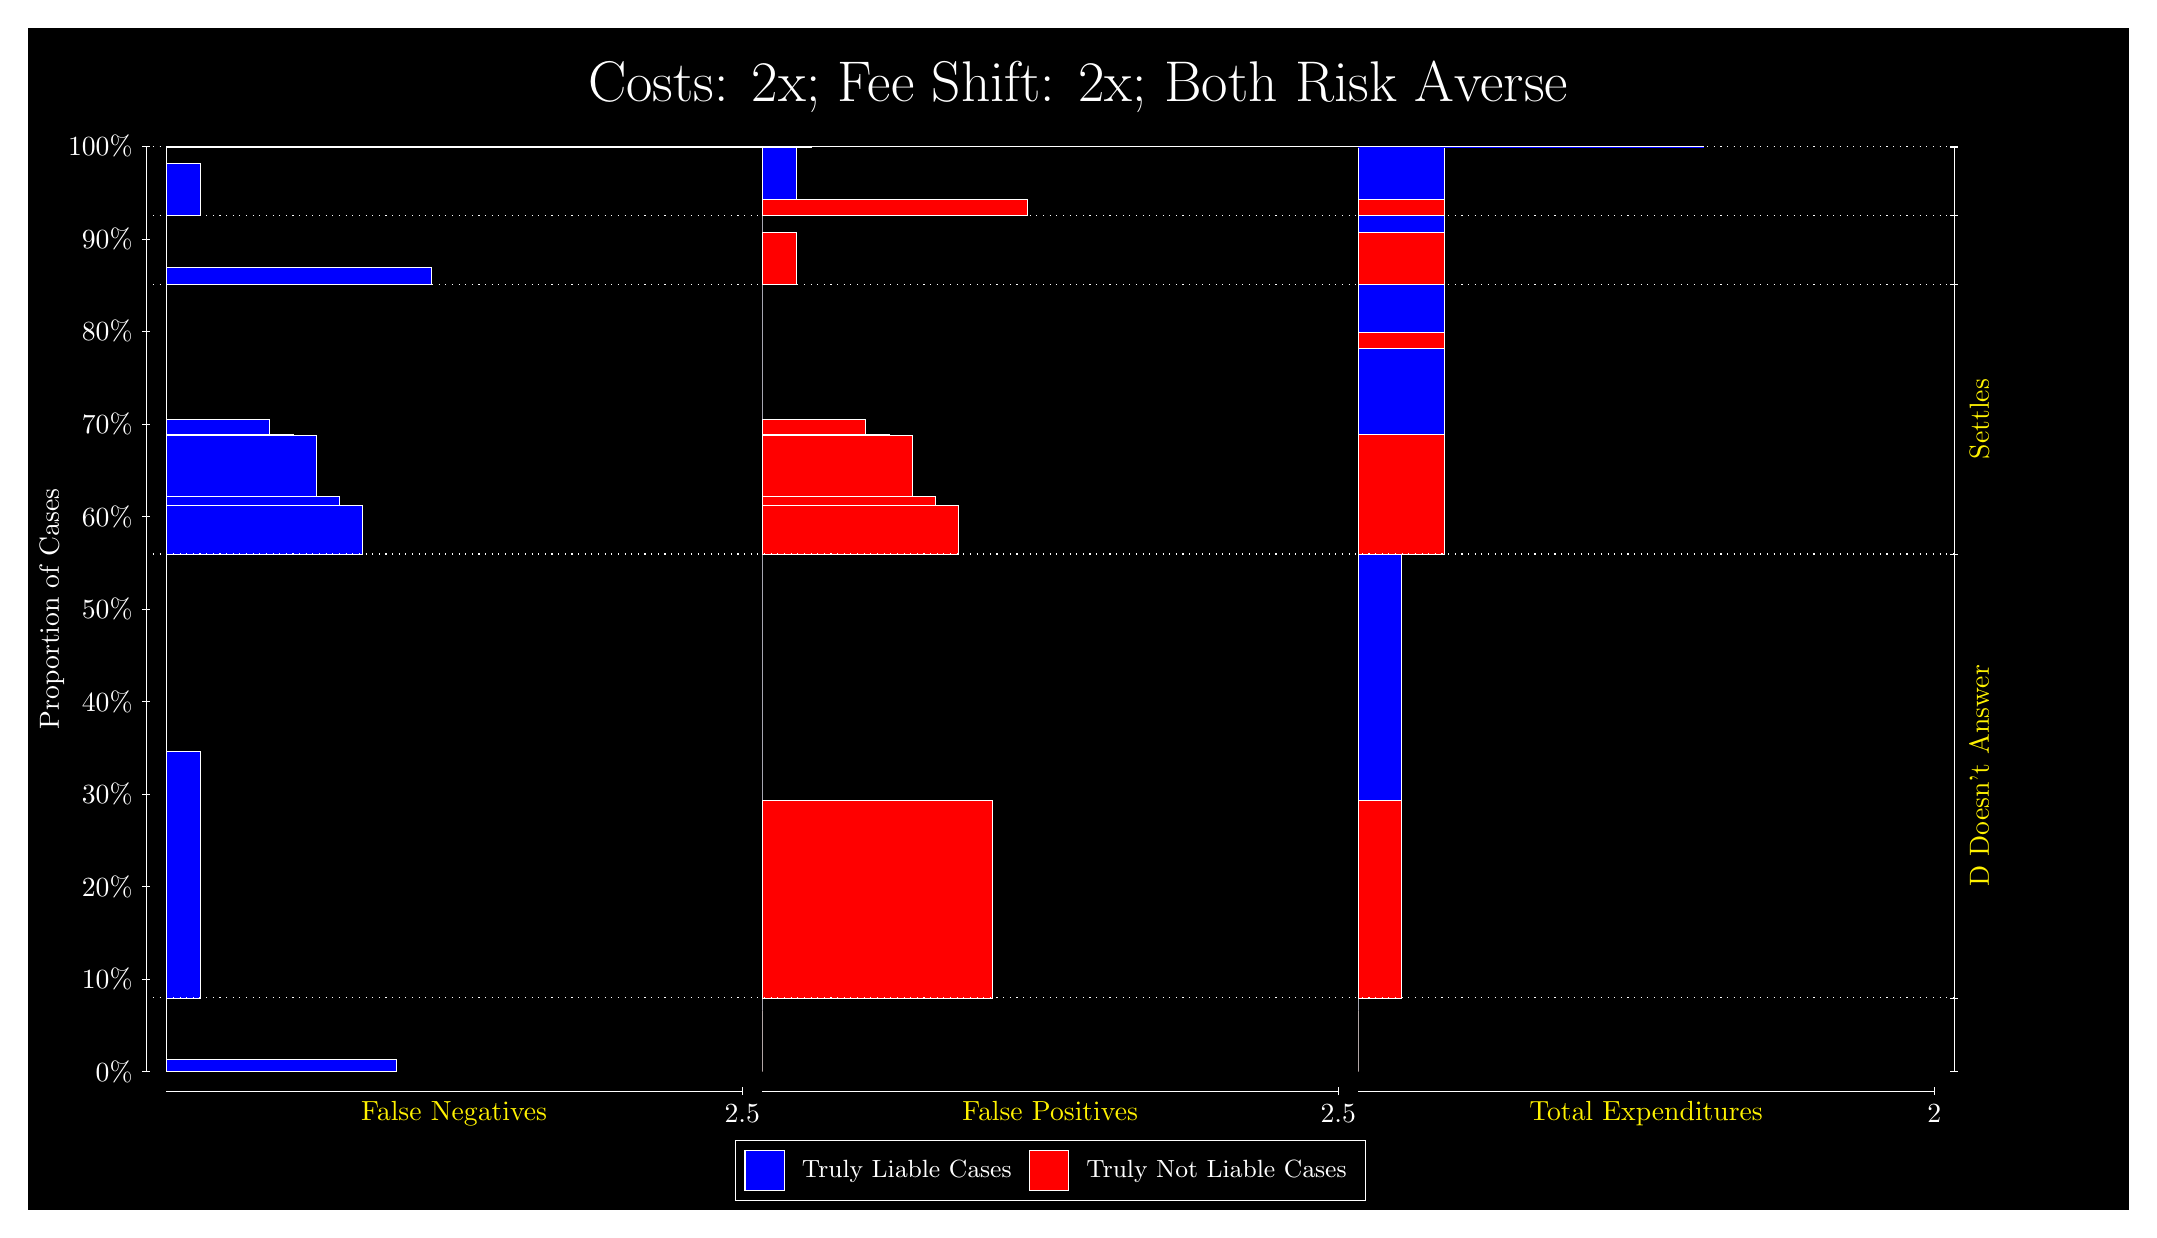
\begin{tikzpicture}
\draw[fill=black] (0,0) rectangle (26.667,15);
\draw[text=white] (0,13.5) rectangle (26.667,15) node[midway] {\huge Costs: 2x; Fee Shift: 2x; Both Risk Averse};
\draw[white, very thin] (1.5,1.75) -- (1.5,13.5);
\node[rotate=90, text=white, anchor=center] at (0.3, 7.625) {Proportion of Cases};
\draw[white, very thin] (1.45,1.75) -- (1.55,1.75);
\node[text=white, anchor=east] at (1.45, 1.75) {0\%};
\draw[white, very thin] (1.45,2.925) -- (1.55,2.925);
\node[text=white, anchor=east] at (1.45, 2.925) {10\%};
\draw[white, very thin] (1.45,4.1) -- (1.55,4.1);
\node[text=white, anchor=east] at (1.45, 4.1) {20\%};
\draw[white, very thin] (1.45,5.275) -- (1.55,5.275);
\node[text=white, anchor=east] at (1.45, 5.275) {30\%};
\draw[white, very thin] (1.45,6.45) -- (1.55,6.45);
\node[text=white, anchor=east] at (1.45, 6.45) {40\%};
\draw[white, very thin] (1.45,7.625) -- (1.55,7.625);
\node[text=white, anchor=east] at (1.45, 7.625) {50\%};
\draw[white, very thin] (1.45,8.8) -- (1.55,8.8);
\node[text=white, anchor=east] at (1.45, 8.8) {60\%};
\draw[white, very thin] (1.45,9.975) -- (1.55,9.975);
\node[text=white, anchor=east] at (1.45, 9.975) {70\%};
\draw[white, very thin] (1.45,11.15) -- (1.55,11.15);
\node[text=white, anchor=east] at (1.45, 11.15) {80\%};
\draw[white, very thin] (1.45,12.325) -- (1.55,12.325);
\node[text=white, anchor=east] at (1.45, 12.325) {90\%};
\draw[white, very thin] (1.45,13.5) -- (1.55,13.5);
\node[text=white, anchor=east] at (1.45, 13.5) {100\%};

\draw[white, very thin] (24.457,1.75) -- (24.457,13.5);
\draw[white, very thin] (24.407,1.75) -- (24.507,1.75);
\node[anchor=west] at (24.407, 1.75) {};
\draw[white, very thin] (24.407,2.6864) -- (24.507,2.6864);
\node[anchor=west] at (24.407, 2.6864) {};
\draw[white, very thin] (24.407,8.3227) -- (24.507,8.3227);
\node[anchor=west] at (24.407, 8.3227) {};
\draw[white, very thin] (24.407,11.75) -- (24.507,11.75);
\node[anchor=west] at (24.407, 11.75) {};
\draw[white, very thin] (24.407,12.622) -- (24.507,12.622);
\node[anchor=west] at (24.407, 12.622) {};
\draw[white, very thin] (24.407,13.494) -- (24.507,13.494);
\node[anchor=west] at (24.407, 13.494) {};
\draw[white, very thin] (24.407,13.497) -- (24.507,13.497);
\node[anchor=west] at (24.407, 13.497) {};
\draw[white, very thin] (24.407,13.5) -- (24.507,13.5);
\node[anchor=west] at (24.407, 13.5) {};

\draw[white, very thin, fill=blue] (1.75,1.75) rectangle (4.6775,1.9112);
\draw[white, very thin, fill=red] (1.75,1.9112) rectangle (1.75,2.6864);
\draw[white, very thin, fill=blue] (1.75,2.6864) rectangle (2.1891,5.8115);
\draw[white, very thin, fill=red] (1.75,5.8115) rectangle (1.75,8.3227);
\draw[white, very thin, fill=blue] (1.75,8.3227) rectangle (4.2384,8.9388);
\draw[white, very thin, fill=blue] (1.75,8.9388) rectangle (3.9457,9.0531);
\draw[white, very thin, fill=blue] (1.75,9.0531) rectangle (3.6529,9.8273);
\draw[white, very thin, fill=blue] (1.75,9.8273) rectangle (3.3602,9.8406);
\draw[white, very thin, fill=blue] (1.75,9.8406) rectangle (3.0674,10.036);
\draw[white, very thin, fill=red] (1.75,10.036) rectangle (1.75,11.75);
\draw[white, very thin, fill=blue] (1.75,11.75) rectangle (5.1167,11.959);
\draw[white, very thin, fill=red] (1.75,11.959) rectangle (1.75,12.622);
\draw[white, very thin, fill=blue] (1.75,12.622) rectangle (2.1891,13.285);
\draw[white, very thin, fill=red] (1.75,13.285) rectangle (1.75,13.494);
\draw[white, very thin, fill=blue] (1.75,13.494) rectangle (9.9471,13.495);
\draw[white, very thin, fill=red] (1.75,13.495) rectangle (1.75,13.497);
\draw[white, very thin, fill=red] (1.75,13.497) rectangle (1.75,13.498);
\draw[white, very thin, fill=blue] (1.75,13.498) rectangle (1.75,13.5);
\draw[white, very thin, fill=red] (9.3189,1.75) rectangle (9.3189,2.5252);
\draw[white, very thin, fill=blue] (9.3189,2.5252) rectangle (9.3189,2.6864);
\draw[white, very thin, fill=red] (9.3189,2.6864) rectangle (12.246,5.1976);
\draw[white, very thin, fill=blue] (9.3189,5.1976) rectangle (9.3189,8.3227);
\draw[white, very thin, fill=red] (9.3189,8.3227) rectangle (11.807,8.9377);
\draw[white, very thin, fill=red] (9.3189,8.9377) rectangle (11.515,9.0533);
\draw[white, very thin, fill=red] (9.3189,9.0533) rectangle (11.222,9.8279);
\draw[white, very thin, fill=red] (9.3189,9.8279) rectangle (10.929,9.841);
\draw[white, very thin, fill=red] (9.3189,9.841) rectangle (10.636,10.036);
\draw[white, very thin, fill=blue] (9.3189,10.036) rectangle (9.3189,11.75);
\draw[white, very thin, fill=red] (9.3189,11.75) rectangle (9.758,12.412);
\draw[white, very thin, fill=blue] (9.3189,12.412) rectangle (9.3189,12.622);
\draw[white, very thin, fill=red] (9.3189,12.622) rectangle (12.686,12.831);
\draw[white, very thin, fill=blue] (9.3189,12.831) rectangle (9.758,13.494);
\draw[white, very thin, fill=red] (9.3189,13.494) rectangle (9.3189,13.496);
\draw[white, very thin, fill=blue] (9.3189,13.496) rectangle (9.3189,13.497);
\draw[white, very thin, fill=red] (9.3189,13.497) rectangle (17.516,13.498);
\draw[white, very thin, fill=blue] (9.3189,13.498) rectangle (14.588,13.5);
\draw[white, very thin, fill=red] (16.888,1.75) rectangle (16.888,2.5252);
\draw[white, very thin, fill=blue] (16.888,2.5252) rectangle (16.888,2.6864);
\draw[white, very thin, fill=red] (16.888,2.6864) rectangle (17.437,5.1976);
\draw[white, very thin, fill=blue] (16.888,5.1976) rectangle (17.437,8.3227);
\draw[white, very thin, fill=red] (16.888,8.3227) rectangle (17.986,9.841);
\draw[white, very thin, fill=blue] (16.888,9.841) rectangle (17.986,10.938);
\draw[white, very thin, fill=red] (16.888,10.938) rectangle (17.986,11.134);
\draw[white, very thin, fill=blue] (16.888,11.134) rectangle (17.986,11.75);
\draw[white, very thin, fill=red] (16.888,11.75) rectangle (17.986,12.412);
\draw[white, very thin, fill=blue] (16.888,12.412) rectangle (17.986,12.622);
\draw[white, very thin, fill=red] (16.888,12.622) rectangle (17.986,12.831);
\draw[white, very thin, fill=blue] (16.888,12.831) rectangle (17.986,13.494);
\draw[white, very thin, fill=red] (16.888,13.494) rectangle (21.279,13.496);
\draw[white, very thin, fill=blue] (16.888,13.496) rectangle (21.279,13.497);
\draw[white, very thin, fill=red] (16.888,13.497) rectangle (21.279,13.498);
\draw[white, very thin, fill=blue] (16.888,13.498) rectangle (21.279,13.5);
\draw[white, dotted] (1.5,2.6864) -- (24.457,2.6864);
\draw[white, dotted] (1.5,8.3227) -- (24.457,8.3227);
\draw[white, dotted] (1.5,11.75) -- (24.457,11.75);
\draw[white, dotted] (1.5,12.622) -- (24.457,12.622);
\draw[white, dotted] (1.5,13.494) -- (24.457,13.494);
\draw[white, dotted] (1.5,13.497) -- (24.457,13.497);
\draw[white, very thin] (1.75,1.5) -- (9.0689,1.5);
\node[text=yellow, anchor=north] at (5.4094, 1.5) {False Negatives};
\draw[white, very thin] (9.0689,1.45) -- (9.0689,1.55);
\node[text=white, anchor=north] at (9.0689, 1.45) {2.5};

\draw[white, very thin] (9.3189,1.5) -- (16.638,1.5);
\node[text=yellow, anchor=north] at (12.978, 1.5) {False Positives};
\draw[white, very thin] (16.638,1.45) -- (16.638,1.55);
\node[text=white, anchor=north] at (16.638, 1.45) {2.5};

\draw[white, very thin] (16.888,1.5) -- (24.207,1.5);
\node[text=yellow, anchor=north] at (20.547, 1.5) {Total Expenditures};
\draw[white, very thin] (24.207,1.45) -- (24.207,1.55);
\node[text=white, anchor=north] at (24.207, 1.45) {2};


\node[text=yellow, centered, rotate=90] at (24.777, 5.5046) {D Doesn't Answer};
\node[text=yellow, centered, rotate=90] at (24.777, 10.036) {Settles};





\draw (12.978300999999998,1.5) node[draw=none] (baseCoordinate) {};
\begin{scope}[align=center]
        \matrix[scale=0.5, draw=white, below=0.5cm of baseCoordinate, nodes={draw}, column sep=0.1cm]{
            \node[rectangle, draw, minimum width=0.5cm, minimum height=0.5cm, fill=blue] {}; &
            \node[draw=none, font=\small, text=white] (B) {Truly Liable Cases}; &
            \node[rectangle, draw, minimum width=0.5cm, minimum height=0.5cm, fill=red] {}; &
            \node[draw=none, font=\small, text=white] (B) {Truly Not Liable Cases}; \\
            };
\end{scope}

\end{tikzpicture}
\end{document}